\PassOptionsToPackage{unicode=true}{hyperref} % options for packages loaded elsewhere
\PassOptionsToPackage{hyphens}{url}
%
\documentclass[]{book}
\usepackage{lmodern}
\usepackage{amssymb,amsmath}
\usepackage{ifxetex,ifluatex}
\usepackage{fixltx2e} % provides \textsubscript
\ifnum 0\ifxetex 1\fi\ifluatex 1\fi=0 % if pdftex
  \usepackage[T1]{fontenc}
  \usepackage[utf8]{inputenc}
  \usepackage{textcomp} % provides euro and other symbols
\else % if luatex or xelatex
  \usepackage{unicode-math}
  \defaultfontfeatures{Ligatures=TeX,Scale=MatchLowercase}
\fi
% use upquote if available, for straight quotes in verbatim environments
\IfFileExists{upquote.sty}{\usepackage{upquote}}{}
% use microtype if available
\IfFileExists{microtype.sty}{%
\usepackage[]{microtype}
\UseMicrotypeSet[protrusion]{basicmath} % disable protrusion for tt fonts
}{}
\IfFileExists{parskip.sty}{%
\usepackage{parskip}
}{% else
\setlength{\parindent}{0pt}
\setlength{\parskip}{6pt plus 2pt minus 1pt}
}
\usepackage{hyperref}
\hypersetup{
            pdftitle={Malaria Disease Detection based on Convolutional Neural Net (CNN)},
            pdfauthor={Dr.K. Palani Thanaraj},
            pdfborder={0 0 0},
            breaklinks=true}
\urlstyle{same}  % don't use monospace font for urls
\usepackage{color}
\usepackage{fancyvrb}
\newcommand{\VerbBar}{|}
\newcommand{\VERB}{\Verb[commandchars=\\\{\}]}
\DefineVerbatimEnvironment{Highlighting}{Verbatim}{commandchars=\\\{\}}
% Add ',fontsize=\small' for more characters per line
\usepackage{framed}
\definecolor{shadecolor}{RGB}{248,248,248}
\newenvironment{Shaded}{\begin{snugshade}}{\end{snugshade}}
\newcommand{\AlertTok}[1]{\textcolor[rgb]{0.94,0.16,0.16}{#1}}
\newcommand{\AnnotationTok}[1]{\textcolor[rgb]{0.56,0.35,0.01}{\textbf{\textit{#1}}}}
\newcommand{\AttributeTok}[1]{\textcolor[rgb]{0.77,0.63,0.00}{#1}}
\newcommand{\BaseNTok}[1]{\textcolor[rgb]{0.00,0.00,0.81}{#1}}
\newcommand{\BuiltInTok}[1]{#1}
\newcommand{\CharTok}[1]{\textcolor[rgb]{0.31,0.60,0.02}{#1}}
\newcommand{\CommentTok}[1]{\textcolor[rgb]{0.56,0.35,0.01}{\textit{#1}}}
\newcommand{\CommentVarTok}[1]{\textcolor[rgb]{0.56,0.35,0.01}{\textbf{\textit{#1}}}}
\newcommand{\ConstantTok}[1]{\textcolor[rgb]{0.00,0.00,0.00}{#1}}
\newcommand{\ControlFlowTok}[1]{\textcolor[rgb]{0.13,0.29,0.53}{\textbf{#1}}}
\newcommand{\DataTypeTok}[1]{\textcolor[rgb]{0.13,0.29,0.53}{#1}}
\newcommand{\DecValTok}[1]{\textcolor[rgb]{0.00,0.00,0.81}{#1}}
\newcommand{\DocumentationTok}[1]{\textcolor[rgb]{0.56,0.35,0.01}{\textbf{\textit{#1}}}}
\newcommand{\ErrorTok}[1]{\textcolor[rgb]{0.64,0.00,0.00}{\textbf{#1}}}
\newcommand{\ExtensionTok}[1]{#1}
\newcommand{\FloatTok}[1]{\textcolor[rgb]{0.00,0.00,0.81}{#1}}
\newcommand{\FunctionTok}[1]{\textcolor[rgb]{0.00,0.00,0.00}{#1}}
\newcommand{\ImportTok}[1]{#1}
\newcommand{\InformationTok}[1]{\textcolor[rgb]{0.56,0.35,0.01}{\textbf{\textit{#1}}}}
\newcommand{\KeywordTok}[1]{\textcolor[rgb]{0.13,0.29,0.53}{\textbf{#1}}}
\newcommand{\NormalTok}[1]{#1}
\newcommand{\OperatorTok}[1]{\textcolor[rgb]{0.81,0.36,0.00}{\textbf{#1}}}
\newcommand{\OtherTok}[1]{\textcolor[rgb]{0.56,0.35,0.01}{#1}}
\newcommand{\PreprocessorTok}[1]{\textcolor[rgb]{0.56,0.35,0.01}{\textit{#1}}}
\newcommand{\RegionMarkerTok}[1]{#1}
\newcommand{\SpecialCharTok}[1]{\textcolor[rgb]{0.00,0.00,0.00}{#1}}
\newcommand{\SpecialStringTok}[1]{\textcolor[rgb]{0.31,0.60,0.02}{#1}}
\newcommand{\StringTok}[1]{\textcolor[rgb]{0.31,0.60,0.02}{#1}}
\newcommand{\VariableTok}[1]{\textcolor[rgb]{0.00,0.00,0.00}{#1}}
\newcommand{\VerbatimStringTok}[1]{\textcolor[rgb]{0.31,0.60,0.02}{#1}}
\newcommand{\WarningTok}[1]{\textcolor[rgb]{0.56,0.35,0.01}{\textbf{\textit{#1}}}}
\usepackage{longtable,booktabs}
% Fix footnotes in tables (requires footnote package)
\IfFileExists{footnote.sty}{\usepackage{footnote}\makesavenoteenv{longtable}}{}
\usepackage{graphicx,grffile}
\makeatletter
\def\maxwidth{\ifdim\Gin@nat@width>\linewidth\linewidth\else\Gin@nat@width\fi}
\def\maxheight{\ifdim\Gin@nat@height>\textheight\textheight\else\Gin@nat@height\fi}
\makeatother
% Scale images if necessary, so that they will not overflow the page
% margins by default, and it is still possible to overwrite the defaults
% using explicit options in \includegraphics[width, height, ...]{}
\setkeys{Gin}{width=\maxwidth,height=\maxheight,keepaspectratio}
\setlength{\emergencystretch}{3em}  % prevent overfull lines
\providecommand{\tightlist}{%
  \setlength{\itemsep}{0pt}\setlength{\parskip}{0pt}}
\setcounter{secnumdepth}{5}
% Redefines (sub)paragraphs to behave more like sections
\ifx\paragraph\undefined\else
\let\oldparagraph\paragraph
\renewcommand{\paragraph}[1]{\oldparagraph{#1}\mbox{}}
\fi
\ifx\subparagraph\undefined\else
\let\oldsubparagraph\subparagraph
\renewcommand{\subparagraph}[1]{\oldsubparagraph{#1}\mbox{}}
\fi

% set default figure placement to htbp
\makeatletter
\def\fps@figure{htbp}
\makeatother

\usepackage{booktabs}
\usepackage[]{natbib}
\bibliographystyle{apalike}

\title{Malaria Disease Detection based on Convolutional Neural Net (CNN)}
\author{Dr.K. Palani Thanaraj}
\date{2020-05-12}

\begin{document}
\maketitle

{
\setcounter{tocdepth}{1}
\tableofcontents
}
\hypertarget{prerequisite}{%
\chapter*{Prerequisite}\label{prerequisite}}
\addcontentsline{toc}{chapter}{Prerequisite}

I am happy to share this free book which is interactive and with python codes for you to get acquaint with the concepts of \textbf{Deep learning (DL)}. We try here to use \texttt{Convolutional\ Neural\ Net\ (CNN)} to classify the malarial cell images. You need to have some prior knowledge about Python programming and Image classification. For practicing the algorithms you can use Google Colab which is absolutely free and the dataset is available in Kaggle at this link:\url{https://www.kaggle.com/iarunava/cell-images-for-detecting-malaria}

\hypertarget{introduction}{%
\chapter{Introduction}\label{introduction}}

Malaria is a deadly disease predominantly caused by a parasite name \texttt{Plasmodium\ falciparum} which is transmitted by mosquito. It shows symptoms such as high fever and chills, which not treated in due time can be fatal. The disease is diagnosed by capturing the cell images of the blood and the presence of parasitic stains can be used to detect the Malarial disease.

\hypertarget{dataset}{%
\section{Dataset}\label{dataset}}

The Kaggle dataset consists of two folders namely \texttt{uninfected} and \texttt{parasitized} cell images. The images are color images which are resized to a dimension of \[128 \times 128\]. The original dataset provides a total of around 25000 images. However, for running our simple DL algorithm we will be using only 100 images for each class.

\hypertarget{python-programming-env}{%
\section{Python Programming ENV}\label{python-programming-env}}

The following section explains about different Python Libraries we would be using for our Malaria detection method. As we are doing the development in the Google Colab, we don't need to install any module here. It is alreadly configured in the Colab ENV, only we have to import the required libraries for our application. The Python codes is grouped into different code chunks for each understanding.

\hypertarget{importing-of-common-array-and-plotting-librariers}{%
\subsection{Importing of common array and plotting librariers}\label{importing-of-common-array-and-plotting-librariers}}

This is for data importing and manipulation using NUMPY and PANDAS. Matplotlib and Seaborn for plotting graphs and images.

\begin{Shaded}
\begin{Highlighting}[]
\ImportTok{import}\NormalTok{ numpy }\ImportTok{as}\NormalTok{ np}
\ImportTok{import}\NormalTok{ pandas }\ImportTok{as}\NormalTok{ pd}
\ImportTok{import}\NormalTok{ matplotlib.pyplot }\ImportTok{as}\NormalTok{ plt}
\ImportTok{from}\NormalTok{ matplotlib }\ImportTok{import}\NormalTok{ style}
\ImportTok{import}\NormalTok{ seaborn }\ImportTok{as}\NormalTok{ sns}
\end{Highlighting}
\end{Shaded}

\hypertarget{importing-of-opencv-and-scikit-learn}{%
\subsection{Importing of OpenCV and Scikit-learn}\label{importing-of-opencv-and-scikit-learn}}

OpenCV and Scikit-learn for image processing and machine learning respectivley.

\begin{Shaded}
\begin{Highlighting}[]
\ImportTok{import}\NormalTok{ cv2 }
\ImportTok{import}\NormalTok{ os}
\ImportTok{from}\NormalTok{ sklearn.feature_extraction }\ImportTok{import}\NormalTok{ image}
\end{Highlighting}
\end{Shaded}

\hypertarget{data-preprocessing}{%
\section{Data Preprocessing}\label{data-preprocessing}}

Here we initialize a set of lists \texttt{X} \& \texttt{Z} for the images and the labels.

\begin{Shaded}
\begin{Highlighting}[]
\ImportTok{from}\NormalTok{ tqdm }\ImportTok{import}\NormalTok{ tqdm}
\NormalTok{X}\OperatorTok{=}\NormalTok{[]}
\NormalTok{Z}\OperatorTok{=}\NormalTok{[]}
\NormalTok{IMG_SIZE}\OperatorTok{=}\DecValTok{128}
\NormalTok{norm_DIR}\OperatorTok{=}\StringTok{'data/uninfected'}
\NormalTok{mal_DIR}\OperatorTok{=}\StringTok{'data/parasitized'}
\end{Highlighting}
\end{Shaded}

\hypertarget{creation-of-lists-for-the-images-and-the-labels}{%
\subsection{Creation of lists for the images and the labels}\label{creation-of-lists-for-the-images-and-the-labels}}

Here we create two functions for creating image lists and labels.

\begin{Shaded}
\begin{Highlighting}[]
\KeywordTok{def}\NormalTok{ assign_label(img,ret_type):}
    \ControlFlowTok{return}\NormalTok{ ret_type}

\KeywordTok{def}\NormalTok{ make_train_data(ret_type,DIR):}
    \ControlFlowTok{for}\NormalTok{ img }\KeywordTok{in}\NormalTok{ tqdm(os.listdir(DIR)):}
\NormalTok{        label}\OperatorTok{=}\NormalTok{assign_label(img,ret_type)}
\NormalTok{        path }\OperatorTok{=}\NormalTok{ os.path.join(DIR,img)}
\NormalTok{        img }\OperatorTok{=}\NormalTok{ cv2.imread(path,cv2.IMREAD_COLOR)}
\NormalTok{        img }\OperatorTok{=}\NormalTok{ cv2.resize(img, (IMG_SIZE,IMG_SIZE))}
        
\NormalTok{        X.append(np.array(img))}
\NormalTok{        Z.append(}\BuiltInTok{str}\NormalTok{(label))}
    
\end{Highlighting}
\end{Shaded}

Here we call the functions to perform the array formation for the images and the labels.

\begin{Shaded}
\begin{Highlighting}[]
\NormalTok{make_train_data(}\StringTok{'Uninfected'}\NormalTok{,norm_DIR)}
\end{Highlighting}
\end{Shaded}

\begin{verbatim}
##   0%|          | 0/100 [00:00<?, ?it/s]100%|##########| 100/100 [00:00<00:00, 1167.75it/s]
\end{verbatim}

\begin{Shaded}
\begin{Highlighting}[]
\BuiltInTok{print}\NormalTok{(}\BuiltInTok{len}\NormalTok{(X))}
\end{Highlighting}
\end{Shaded}

\begin{verbatim}
## 100
\end{verbatim}

\begin{Shaded}
\begin{Highlighting}[]
\NormalTok{make_train_data(}\StringTok{'Parasitized'}\NormalTok{,mal_DIR)}
\end{Highlighting}
\end{Shaded}

\begin{verbatim}
##   0%|          | 0/100 [00:00<?, ?it/s]100%|##########| 100/100 [00:00<00:00, 1553.07it/s]
\end{verbatim}

\begin{Shaded}
\begin{Highlighting}[]
\BuiltInTok{print}\NormalTok{(}\BuiltInTok{len}\NormalTok{(X))}
\end{Highlighting}
\end{Shaded}

\begin{verbatim}
## 200
\end{verbatim}

\hypertarget{plotting-of-the-sample-images}{%
\section{Plotting of the sample images}\label{plotting-of-the-sample-images}}

Here we plot some of the cell images of malarial and uninfected person blood.

\begin{Shaded}
\begin{Highlighting}[]
\ImportTok{import}\NormalTok{ random }\ImportTok{as}\NormalTok{ rn}
\NormalTok{fig,ax}\OperatorTok{=}\NormalTok{plt.subplots(}\DecValTok{2}\NormalTok{,}\DecValTok{2}\NormalTok{)}
\NormalTok{fig.set_size_inches(}\DecValTok{6}\NormalTok{,}\DecValTok{6}\NormalTok{)}
\ControlFlowTok{for}\NormalTok{ i }\KeywordTok{in} \BuiltInTok{range}\NormalTok{(}\DecValTok{2}\NormalTok{):}
    \ControlFlowTok{for}\NormalTok{ j }\KeywordTok{in} \BuiltInTok{range}\NormalTok{ (}\DecValTok{2}\NormalTok{):}
\NormalTok{        l}\OperatorTok{=}\NormalTok{rn.randint(}\DecValTok{0}\NormalTok{,}\BuiltInTok{len}\NormalTok{(Z))}
\NormalTok{        ax[i,j].imshow(X[l])}
\NormalTok{        ax[i,j].set_title(}\StringTok{'Ret: '}\OperatorTok{+}\NormalTok{Z[l])}
\NormalTok{        plt.tight_layout()}
        
\end{Highlighting}
\end{Shaded}

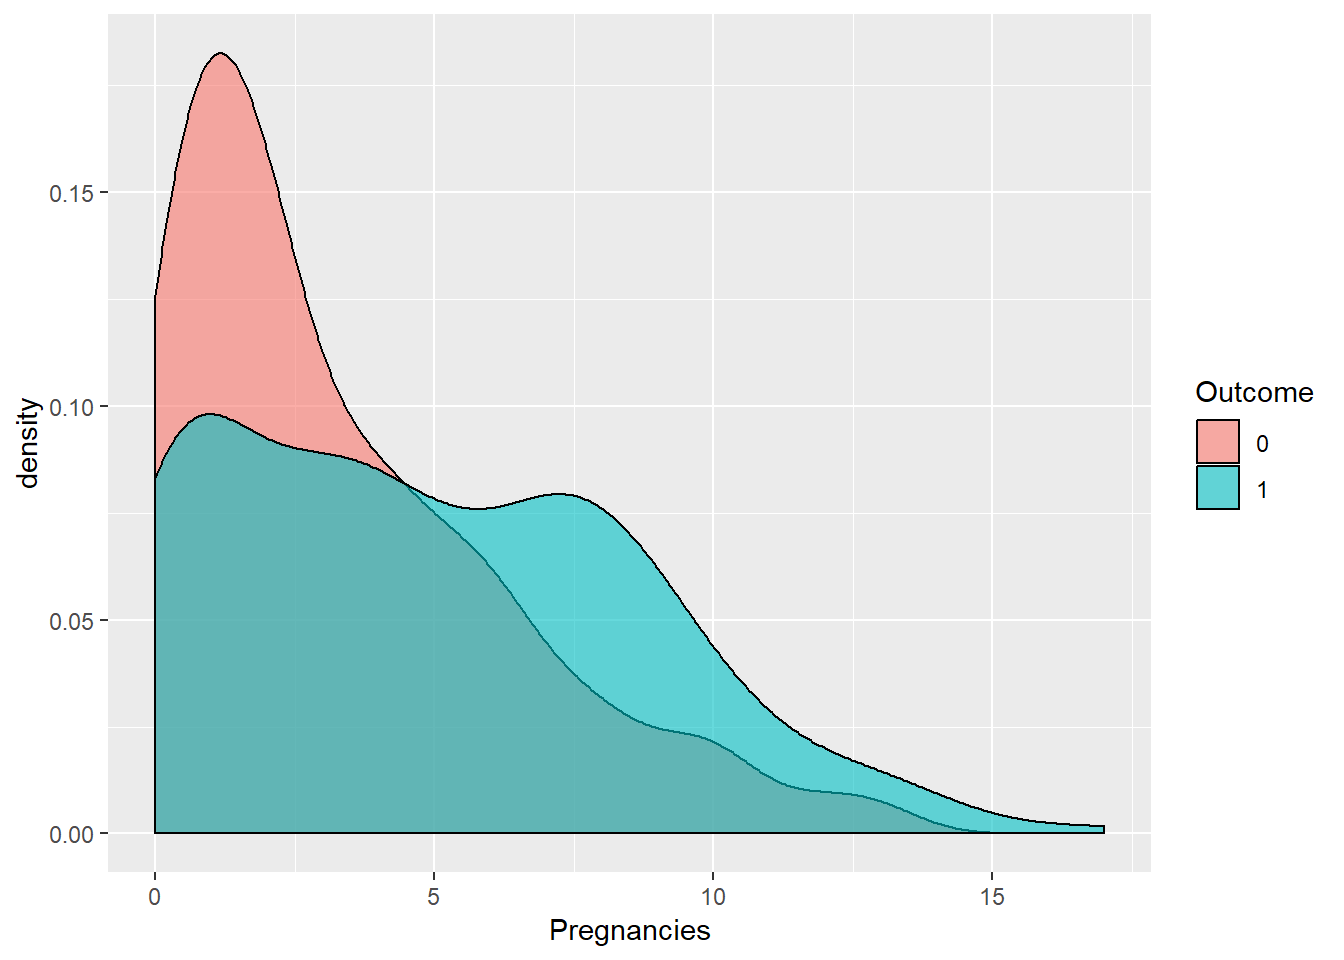
\includegraphics{book1_files/figure-latex/unnamed-chunk-6-1.pdf}
\#\# Label Encoding
Here is a label preprocessing where we perform one hot encoding of the labels.

\begin{Shaded}
\begin{Highlighting}[]
\ImportTok{from}\NormalTok{ sklearn.preprocessing }\ImportTok{import}\NormalTok{ LabelEncoder}
\ImportTok{import}\NormalTok{ tensorflow }
\ImportTok{from}\NormalTok{ tensorflow.keras.utils }\ImportTok{import}\NormalTok{ to_categorical}

\NormalTok{le}\OperatorTok{=}\NormalTok{LabelEncoder()}
\NormalTok{Y}\OperatorTok{=}\NormalTok{le.fit_transform(Z)}
\NormalTok{Y}\OperatorTok{=}\NormalTok{to_categorical(Y,}\DecValTok{2}\NormalTok{)}
\NormalTok{X}\OperatorTok{=}\NormalTok{np.array(X)}
\NormalTok{X}\OperatorTok{=}\NormalTok{X}\OperatorTok{/}\DecValTok{255}
\end{Highlighting}
\end{Shaded}

\hypertarget{data-splitting}{%
\section{Data Splitting}\label{data-splitting}}

Here we perform the splitting of the dataset into \texttt{Training\ (75\%)} and \texttt{Testing\ (25\%)} datasets.

\begin{Shaded}
\begin{Highlighting}[]
\ImportTok{from}\NormalTok{ sklearn.model_selection }\ImportTok{import}\NormalTok{ train_test_split}
\ImportTok{from}\NormalTok{ sklearn.metrics }\ImportTok{import}\NormalTok{ accuracy_score,precision_score,recall_score,confusion_matrix,roc_curve,roc_auc_score}

\NormalTok{x_train,x_test,y_train,y_test}\OperatorTok{=}\NormalTok{train_test_split(X,Y,test_size}\OperatorTok{=}\FloatTok{0.25}\NormalTok{,random_state}\OperatorTok{=}\DecValTok{42}\NormalTok{)}
\BuiltInTok{print}\NormalTok{(x_train.shape)}
\end{Highlighting}
\end{Shaded}

\begin{verbatim}
## (150, 128, 128, 3)
\end{verbatim}

\begin{Shaded}
\begin{Highlighting}[]
\BuiltInTok{print}\NormalTok{(y_train.shape)}
\end{Highlighting}
\end{Shaded}

\begin{verbatim}
## (150, 2)
\end{verbatim}

\begin{Shaded}
\begin{Highlighting}[]
\BuiltInTok{print}\NormalTok{(x_test.shape)}
\end{Highlighting}
\end{Shaded}

\begin{verbatim}
## (50, 128, 128, 3)
\end{verbatim}

\begin{Shaded}
\begin{Highlighting}[]
\BuiltInTok{print}\NormalTok{(y_test.shape)}
\end{Highlighting}
\end{Shaded}

\begin{verbatim}
## (50, 2)
\end{verbatim}

\hypertarget{deep-learning-model-based-on-cnn}{%
\section{Deep Learning Model based on CNN}\label{deep-learning-model-based-on-cnn}}

This section explains about our deep learning model based on CNN. Here we will use 4 Convolutional blocks and 4 Max-Pooling blocks. Finally we will be having a classification layer based on SOFTMAX function for classifying the cell images as \texttt{uninfected} or \texttt{parasitized}.

\begin{Shaded}
\begin{Highlighting}[]
\CommentTok{# # modelling starts using a CNN.}
\ImportTok{from}\NormalTok{ tensorflow.keras.models }\ImportTok{import}\NormalTok{ Sequential}
\ImportTok{import}\NormalTok{ tensorflow }\ImportTok{as}\NormalTok{ tf}

\NormalTok{model }\OperatorTok{=}\NormalTok{ Sequential()}
\NormalTok{model.add(tf.keras.layers.Conv2D(filters }\OperatorTok{=} \DecValTok{32}\NormalTok{, kernel_size }\OperatorTok{=}\NormalTok{ (}\DecValTok{5}\NormalTok{,}\DecValTok{5}\NormalTok{),padding }\OperatorTok{=} \StringTok{'Same'}\NormalTok{,activation }\OperatorTok{=}\StringTok{'relu'}\NormalTok{, input_shape }\OperatorTok{=}\NormalTok{ (}\DecValTok{128}\NormalTok{,}\DecValTok{128}\NormalTok{,}\DecValTok{3}\NormalTok{)))}
\NormalTok{model.add(tf.keras.layers.MaxPooling2D(pool_size}\OperatorTok{=}\NormalTok{(}\DecValTok{2}\NormalTok{,}\DecValTok{2}\NormalTok{)))}


\NormalTok{model.add(tf.keras.layers.Conv2D(filters }\OperatorTok{=} \DecValTok{64}\NormalTok{, kernel_size }\OperatorTok{=}\NormalTok{ (}\DecValTok{3}\NormalTok{,}\DecValTok{3}\NormalTok{),padding }\OperatorTok{=} \StringTok{'Same'}\NormalTok{,activation }\OperatorTok{=}\StringTok{'relu'}\NormalTok{))}
\NormalTok{model.add(tf.keras.layers.MaxPooling2D(pool_size}\OperatorTok{=}\NormalTok{(}\DecValTok{2}\NormalTok{,}\DecValTok{2}\NormalTok{), strides}\OperatorTok{=}\NormalTok{(}\DecValTok{2}\NormalTok{,}\DecValTok{2}\NormalTok{)))}
 

\NormalTok{model.add(tf.keras.layers.Conv2D(filters }\OperatorTok{=}\DecValTok{96}\NormalTok{, kernel_size }\OperatorTok{=}\NormalTok{ (}\DecValTok{3}\NormalTok{,}\DecValTok{3}\NormalTok{),padding }\OperatorTok{=} \StringTok{'Same'}\NormalTok{,activation }\OperatorTok{=}\StringTok{'relu'}\NormalTok{))}
\NormalTok{model.add(tf.keras.layers.MaxPooling2D(pool_size}\OperatorTok{=}\NormalTok{(}\DecValTok{2}\NormalTok{,}\DecValTok{2}\NormalTok{), strides}\OperatorTok{=}\NormalTok{(}\DecValTok{2}\NormalTok{,}\DecValTok{2}\NormalTok{)))}

\NormalTok{model.add(tf.keras.layers.Conv2D(filters }\OperatorTok{=} \DecValTok{96}\NormalTok{, kernel_size }\OperatorTok{=}\NormalTok{ (}\DecValTok{3}\NormalTok{,}\DecValTok{3}\NormalTok{),padding }\OperatorTok{=} \StringTok{'Same'}\NormalTok{,activation }\OperatorTok{=}\StringTok{'relu'}\NormalTok{))}
\NormalTok{model.add(tf.keras.layers.MaxPooling2D(pool_size}\OperatorTok{=}\NormalTok{(}\DecValTok{2}\NormalTok{,}\DecValTok{2}\NormalTok{), strides}\OperatorTok{=}\NormalTok{(}\DecValTok{2}\NormalTok{,}\DecValTok{2}\NormalTok{)))}

\NormalTok{model.add(tf.keras.layers.Flatten())}
\NormalTok{model.add(tf.keras.layers.Dense(}\DecValTok{512}\NormalTok{,activation }\OperatorTok{=}\StringTok{'relu'}\NormalTok{))}
\NormalTok{model.add(tf.keras.layers.Dense(}\DecValTok{2}\NormalTok{, activation }\OperatorTok{=} \StringTok{"softmax"}\NormalTok{))}
\end{Highlighting}
\end{Shaded}

\hypertarget{deep-learning-model-architecture}{%
\section{Deep learning model architecture}\label{deep-learning-model-architecture}}

This sections shows the DL model based on CNN for cell image classification. The number of parametes are also provided here.

\begin{Shaded}
\begin{Highlighting}[]
\NormalTok{model.summary()}
\end{Highlighting}
\end{Shaded}

\begin{verbatim}
## Model: "sequential_1"
## _________________________________________________________________
## Layer (type)                 Output Shape              Param #   
## =================================================================
## conv2d_4 (Conv2D)            (None, 128, 128, 32)      2432      
## _________________________________________________________________
## max_pooling2d_4 (MaxPooling2 (None, 64, 64, 32)        0         
## _________________________________________________________________
## conv2d_5 (Conv2D)            (None, 64, 64, 64)        18496     
## _________________________________________________________________
## max_pooling2d_5 (MaxPooling2 (None, 32, 32, 64)        0         
## _________________________________________________________________
## conv2d_6 (Conv2D)            (None, 32, 32, 96)        55392     
## _________________________________________________________________
## max_pooling2d_6 (MaxPooling2 (None, 16, 16, 96)        0         
## _________________________________________________________________
## conv2d_7 (Conv2D)            (None, 16, 16, 96)        83040     
## _________________________________________________________________
## max_pooling2d_7 (MaxPooling2 (None, 8, 8, 96)          0         
## _________________________________________________________________
## flatten_1 (Flatten)          (None, 6144)              0         
## _________________________________________________________________
## dense_2 (Dense)              (None, 512)               3146240   
## _________________________________________________________________
## dense_3 (Dense)              (None, 2)                 1026      
## =================================================================
## Total params: 3,306,626
## Trainable params: 3,306,626
## Non-trainable params: 0
## _________________________________________________________________
\end{verbatim}

\hypertarget{model-compile}{%
\section{Model Compile}\label{model-compile}}

Here we compile the CNN model for checking any errors and initialize the ADAM optimizer. We have used \texttt{Cross-Entropy} has our loss function.

\begin{Shaded}
\begin{Highlighting}[]
\NormalTok{model.}\BuiltInTok{compile}\NormalTok{(optimizer}\OperatorTok{=}\NormalTok{tf.keras.optimizers.Adam(lr}\OperatorTok{=}\FloatTok{0.001}\NormalTok{),loss}\OperatorTok{=}\StringTok{'categorical_crossentropy'}\NormalTok{,metrics}\OperatorTok{=}\NormalTok{[}\StringTok{'accuracy'}\NormalTok{])}
\end{Highlighting}
\end{Shaded}

\hypertarget{model-training}{%
\section{Model Training}\label{model-training}}

Here we train our DL model using \texttt{FIT} function. We use batch size of 4 and training epochs of 5

\begin{Shaded}
\begin{Highlighting}[]
\BuiltInTok{print}\NormalTok{(}\StringTok{'# Fit model on training data'}\NormalTok{)}
\end{Highlighting}
\end{Shaded}

\begin{Shaded}
\begin{Highlighting}[]
\NormalTok{history }\OperatorTok{=}\NormalTok{ model.fit(x_train, y_train,}
\NormalTok{                    batch_size}\OperatorTok{=}\DecValTok{4}\NormalTok{,}
\NormalTok{                    epochs}\OperatorTok{=}\DecValTok{10}\NormalTok{,}
                    \CommentTok{# We pass some validation for}
                    \CommentTok{# monitoring validation loss and metrics}
                    \CommentTok{# at the end of each epoch}
\NormalTok{                    validation_data}\OperatorTok{=}\NormalTok{(x_test, y_test))}
                    
\end{Highlighting}
\end{Shaded}

\hypertarget{plotting-variables-of-training-sequence}{%
\section{Plotting Variables of Training Sequence}\label{plotting-variables-of-training-sequence}}

\begin{Shaded}
\begin{Highlighting}[]
\BuiltInTok{print}\NormalTok{(history.history.keys())}
\end{Highlighting}
\end{Shaded}

\begin{verbatim}
## dict_keys(['loss', 'acc', 'val_loss', 'val_acc'])
\end{verbatim}

\hypertarget{training-sequence-accuracy}{%
\section{Training Sequence-Accuracy}\label{training-sequence-accuracy}}

The plot showing the accuracy of the DL model during training and testing phase.

\begin{Shaded}
\begin{Highlighting}[]
\CommentTok{# summarize history for accuracy}
\NormalTok{plt.rcParams[}\StringTok{"figure.dpi"}\NormalTok{] }\OperatorTok{=} \DecValTok{200}
\NormalTok{plt.rcParams[}\StringTok{"figure.figsize"}\NormalTok{] }\OperatorTok{=}\NormalTok{ (}\DecValTok{4}\NormalTok{,}\DecValTok{3}\NormalTok{)}
\NormalTok{plt.plot(history.history[}\StringTok{'acc'}\NormalTok{])}
\NormalTok{plt.plot(history.history[}\StringTok{'val_acc'}\NormalTok{])}
\NormalTok{plt.title(}\StringTok{'model accuracy'}\NormalTok{)}
\NormalTok{plt.ylabel(}\StringTok{'accuracy'}\NormalTok{)}
\NormalTok{plt.xlabel(}\StringTok{'epoch'}\NormalTok{)}
\NormalTok{plt.xlim([}\BuiltInTok{min}\NormalTok{(plt.ylim()),}\DecValTok{10}\NormalTok{])}
\end{Highlighting}
\end{Shaded}

\begin{verbatim}
## (0.4350000098347664, 10)
\end{verbatim}

\begin{Shaded}
\begin{Highlighting}[]
\NormalTok{plt.legend([}\StringTok{'train'}\NormalTok{, }\StringTok{'test'}\NormalTok{], loc}\OperatorTok{=}\StringTok{'upper left'}\NormalTok{)}
\NormalTok{plt.show()}
\end{Highlighting}
\end{Shaded}

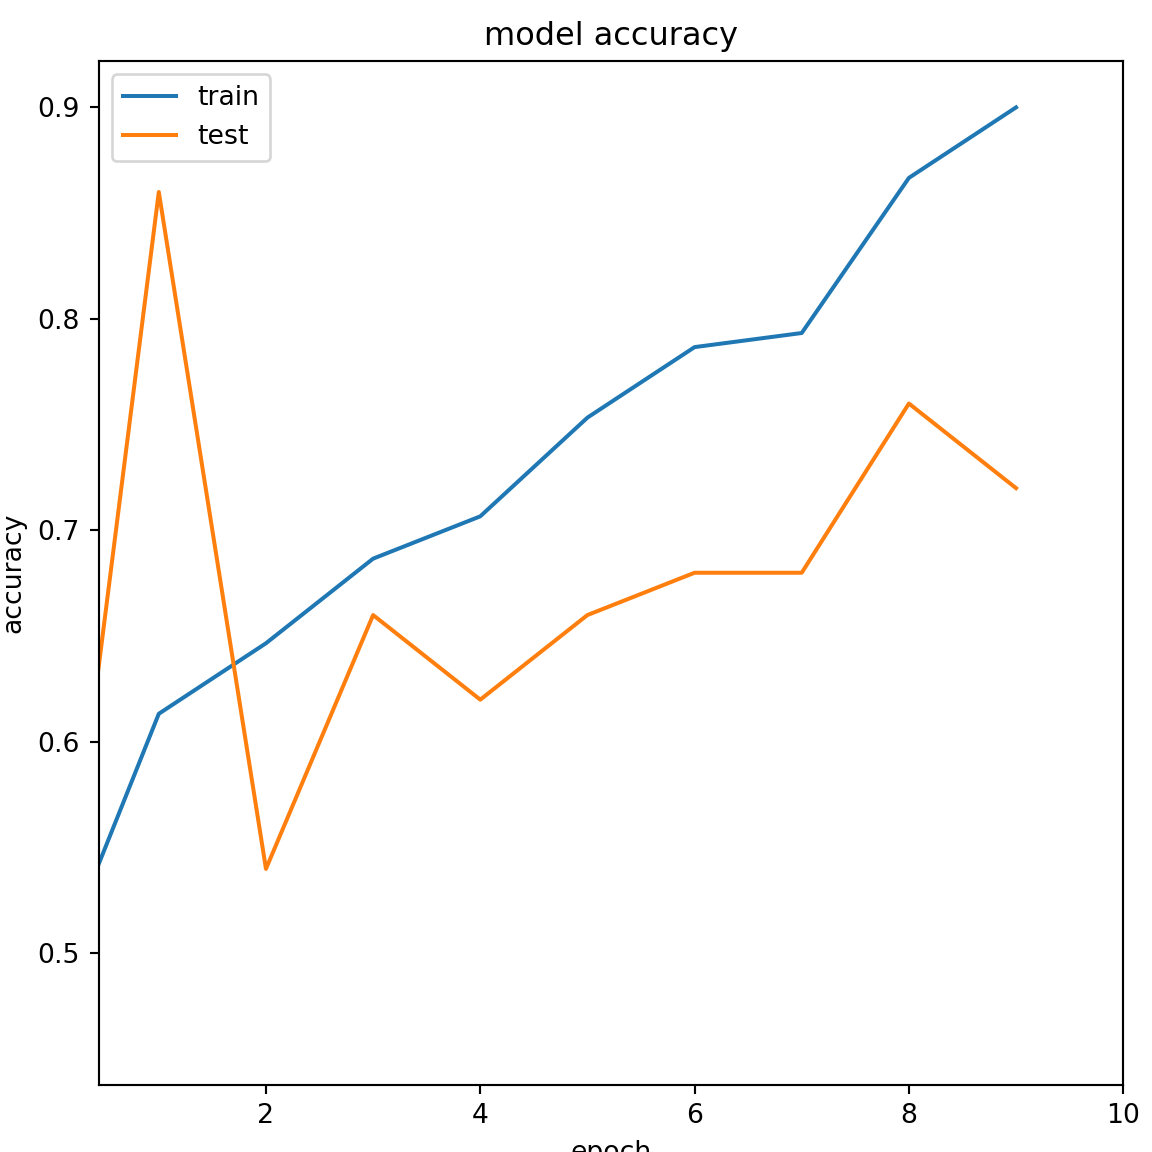
\includegraphics{book1_files/figure-latex/unnamed-chunk-14-1.pdf}

\hypertarget{training-sequence-loss-function}{%
\section{Training Sequence-Loss Function}\label{training-sequence-loss-function}}

The plot showing the loss of the DL model during training and testing phase.

\begin{Shaded}
\begin{Highlighting}[]

\CommentTok{# summarize history for loss}
\NormalTok{plt.plot(history.history[}\StringTok{'loss'}\NormalTok{])}
\NormalTok{plt.plot(history.history[}\StringTok{'val_loss'}\NormalTok{])}
\NormalTok{plt.rcParams[}\StringTok{"figure.figsize"}\NormalTok{] }\OperatorTok{=}\NormalTok{ (}\DecValTok{4}\NormalTok{,}\DecValTok{3}\NormalTok{)}

\NormalTok{plt.title(}\StringTok{'model loss'}\NormalTok{)}
\NormalTok{plt.ylabel(}\StringTok{'loss'}\NormalTok{)}
\NormalTok{plt.xlabel(}\StringTok{'epoch'}\NormalTok{)}
\NormalTok{plt.xlim([}\BuiltInTok{min}\NormalTok{(plt.ylim()),}\DecValTok{10}\NormalTok{])}
\end{Highlighting}
\end{Shaded}

\begin{verbatim}
## (0.04585375600587577, 10)
\end{verbatim}

\begin{Shaded}
\begin{Highlighting}[]
\NormalTok{plt.legend([}\StringTok{'train'}\NormalTok{, }\StringTok{'test'}\NormalTok{], loc}\OperatorTok{=}\StringTok{'upper left'}\NormalTok{)}
\NormalTok{plt.show()}
\end{Highlighting}
\end{Shaded}

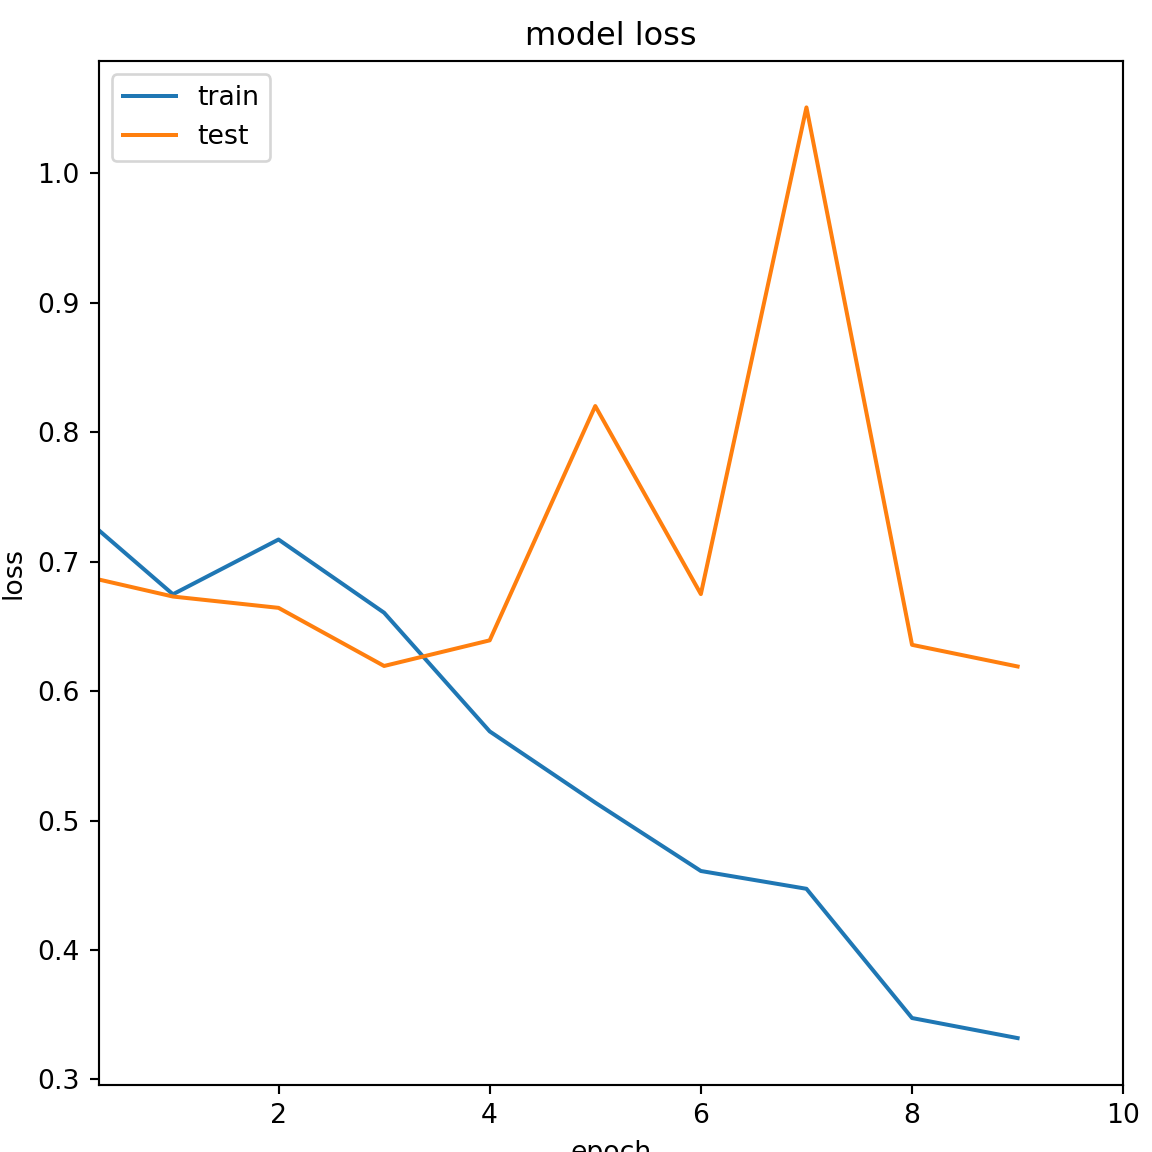
\includegraphics{book1_files/figure-latex/unnamed-chunk-15-1.pdf}

\hypertarget{model-prediction-for-evaluation}{%
\section{Model Prediction for Evaluation}\label{model-prediction-for-evaluation}}

\begin{Shaded}
\begin{Highlighting}[]
\NormalTok{predictions }\OperatorTok{=}\NormalTok{ model.predict(x_test)}
\NormalTok{predicted_classes }\OperatorTok{=}\NormalTok{ np.argmax(predictions, axis}\OperatorTok{=}\DecValTok{1}\NormalTok{)}
\NormalTok{true_classes}\OperatorTok{=}\NormalTok{np.argmax(y_test,axis}\OperatorTok{=}\DecValTok{1}\NormalTok{)}
\end{Highlighting}
\end{Shaded}

\hypertarget{testing-accuracy-and-confusion-matrix}{%
\section{Testing Accuracy and Confusion Matrix}\label{testing-accuracy-and-confusion-matrix}}

\begin{Shaded}
\begin{Highlighting}[]
\ImportTok{import}\NormalTok{ sklearn.metrics }\ImportTok{as}\NormalTok{ metrics}
\ImportTok{from}\NormalTok{ sklearn.metrics }\ImportTok{import}\NormalTok{ confusion_matrix}
\BuiltInTok{print}\NormalTok{(}\StringTok{'Accuracy for malaria disease classifier='}\NormalTok{,metrics.accuracy_score(predicted_classes,true_classes))}
\end{Highlighting}
\end{Shaded}

\begin{verbatim}
## Accuracy for malaria disease classifier= 0.94
\end{verbatim}

\begin{Shaded}
\begin{Highlighting}[]
\BuiltInTok{print}\NormalTok{(}\StringTok{'Confusion matrix=}\CharTok{\textbackslash{}n}\StringTok{'}\NormalTok{,confusion_matrix(true_classes, predicted_classes))}
\end{Highlighting}
\end{Shaded}

\begin{verbatim}
## Confusion matrix=
##  [[21  2]
##  [ 1 26]]
\end{verbatim}

\hypertarget{roc-plot-of-the-dl-model}{%
\section{ROC plot of the DL model}\label{roc-plot-of-the-dl-model}}

\begin{Shaded}
\begin{Highlighting}[]
\ImportTok{from}\NormalTok{ sklearn.metrics }\ImportTok{import}\NormalTok{ roc_curve, auc}
\NormalTok{fpr_keras, tpr_keras, thresholds_keras }\OperatorTok{=}\NormalTok{ roc_curve(true_classes, predictions[:,}\DecValTok{1}\NormalTok{])}
\NormalTok{auc_rf }\OperatorTok{=}\NormalTok{ auc(fpr_keras, tpr_keras)}
\NormalTok{auc_rf}
\end{Highlighting}
\end{Shaded}

\begin{verbatim}
## 0.9533011272141707
\end{verbatim}

\begin{Shaded}
\begin{Highlighting}[]
\NormalTok{plt.rcParams[}\StringTok{"figure.figsize"}\NormalTok{] }\OperatorTok{=}\NormalTok{ (}\DecValTok{4}\NormalTok{,}\DecValTok{3}\NormalTok{)}
\NormalTok{plt.figure(}\DecValTok{1}\NormalTok{)}
\NormalTok{plt.plot([}\DecValTok{0}\NormalTok{, }\DecValTok{1}\NormalTok{], [}\DecValTok{0}\NormalTok{, }\DecValTok{1}\NormalTok{], }\StringTok{'k--'}\NormalTok{)}
\NormalTok{plt.plot(fpr_keras, tpr_keras, label}\OperatorTok{=}\StringTok{'ROC (area = }\SpecialCharTok{\{:.3f\}}\StringTok{)'}\NormalTok{.}\BuiltInTok{format}\NormalTok{(auc_rf))}
\NormalTok{plt.xlabel(}\StringTok{'False positive rate'}\NormalTok{)}
\NormalTok{plt.ylabel(}\StringTok{'True positive rate'}\NormalTok{)}
\NormalTok{plt.title(}\StringTok{'ROC curve'}\NormalTok{)}
\NormalTok{plt.legend(loc}\OperatorTok{=}\StringTok{'best'}\NormalTok{)}
\NormalTok{plt.show()}
\end{Highlighting}
\end{Shaded}

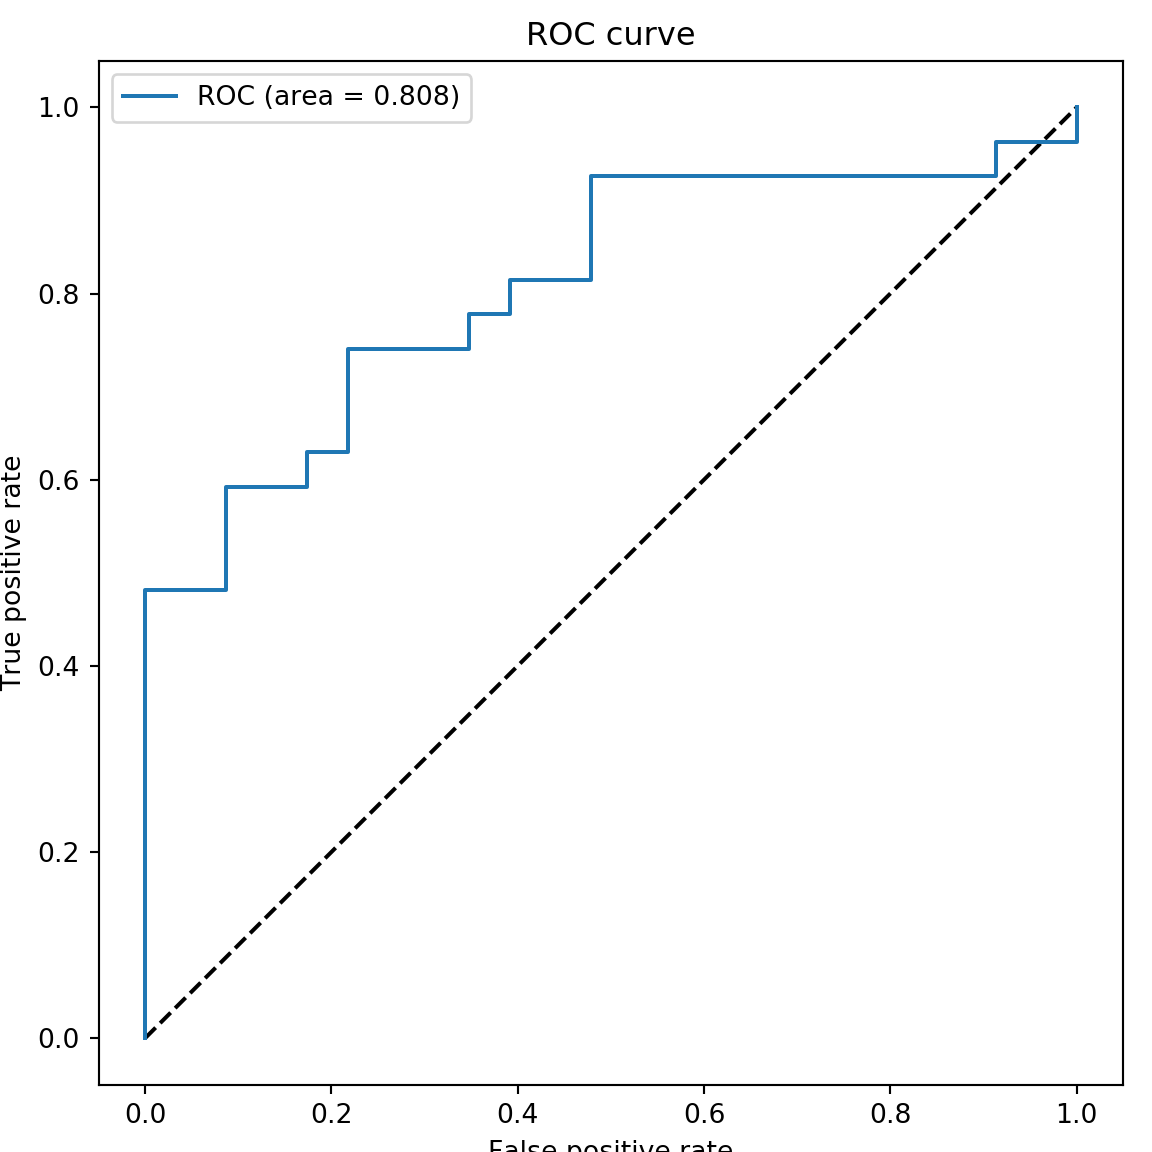
\includegraphics{book1_files/figure-latex/unnamed-chunk-18-1.pdf}

Some papers for related information on Deep Learning Technologies:

\begin{itemize}
\tightlist
\item
  \citep{bhandary2020deep}
\item
  \citep{lakshmi2019convolutional}
\item
  \citep{xie2015}
\end{itemize}

\hypertarget{references}{%
\chapter*{References}\label{references}}
\addcontentsline{toc}{chapter}{References}

\bibliography{book.bib,packages.bib}

\end{document}
